% mnras_template.tex
%
% LaTeX template for creating an MNRAS paper
%
% v3.0 released 14 May 2015
% (version numbers match those of mnras.cls)
%
% Copyright (C) Royal Astronomical Society 2015
% Authors:
% Keith T. Smith (Royal Astronomical Society)

% Change log
%
% v3.0 May 2015
%    Renamed to match the new package name
%    Version number matches mnras.cls
%    A few minor tweaks to wording
% v1.0 September 2013
%    Beta testing only - never publicly released
%    First version: a simple (ish) template for creating an MNRAS paper

%%%%%%%%%%%%%%%%%%%%%%%%%%%%%%%%%%%%%%%%%%%%%%%%%%
% Basic setup. Most papers should leave these options alone.
\documentclass[a4paper,fleqn,usenatbib]{mnras}
\voffset -1.0true cm


% MNRAS is set in Times font. If you don't have this installed (most LaTeX
% installations will be fine) or prefer the old Computer Modern fonts, comment
% out the following line
%\usepackage{newtxtext,newtxmath}
% Depending on your LaTeX fonts installation, you might get better results with one of these:
\usepackage{mathptmx}
%\usepackage{txfonts}
%\usepackage{times}

% Use vector fonts, so it zooms properly in on-screen viewing software
% Don't change these lines unless you know what you are doing
\usepackage[T1]{fontenc}
\usepackage{ae,aecompl}


%%%%% AUTHORS - PLACE YOUR OWN PACKAGES HERE %%%%%

% Only include extra packages if you really need them. Common packages are:
\usepackage{graphicx}	% Including figure files
\usepackage{amsmath}	% Advanced maths commands
\usepackage{amssymb}	% Extra maths symbols
\usepackage{aas_macros}
\usepackage{longtable}
\usepackage{color}
\usepackage{times}
\usepackage{multirow}
\usepackage[dvipsnames]{xcolor}
%\usepackage{caption}

%\captionsetup{compatibility=false}


%%%%%%%%%%%%%%%%%%%%%%%%%%%%%%%%%%%%%%%%%%%%%%%%%%

%%%%% AUTHORS - PLACE YOUR OWN COMMANDS HERE %%%%%

% Please keep new commands to a minimum, and use \newcommand not \def to avoid
% overwriting existing commands. Example:
%\newcommand{\pcm}{\,cm$^{-2}$}	% per cm-squared
\newcommand{\NBeam}{6100}
\newcommand{\us}{$\mu$s}
%\newcommand{\dg}{$^{\circ}$}
\newcommand{\TODO}{\textcolor{red}{TODO}}
\newcommand\red[1]{{\color{red}#1}}
\newcommand{\ps}{$\Phi_{\text{s}}$}
\newcommand{\nobracket}{}
\newcommand{\tmop}[1]{\ensuremath{\operatorname{#1}}}
%\newcommand\footnoteref[1]{\protected@xdef\@thefnmark{\ref{#1}}\@footnotemark}

%%%%%%%%%%%%%%%%%%%%%%%%%%%%%%%%%%%%%%%%%%%%%%%%%%

%%%%%%%%%%%%%%%%%%% TITLE PAGE %%%%%%%%%%%%%%%%%%%

% Title of the paper, and the short title which is used in the headers.
% Keep the title short and informative.
\title[SPAN512]{The SPAN512 mid-latitude pulsar survey: set-up and initial discoveries}

% The list of authors, and the short list which is used in the headers.
% If you need two or more lines of authors, add an extra line using \newauthor
\author[G. Desvignes et al.]{\parbox{\textwidth}{G.~Desvignes,$^{1}$\thanks{E-mail:gdesvignes@mpifr-bonn.mpg.de}
 I.~Cognard,$^{2,3}$
 D.~Champion,$^{1}$
 P.~Lazarus,$^{1}$
 P.~Lespagnol,$^{3}$
 F.~Octau,$^{2}$
 D.~Smith,$^{4}$
 }
\vspace{0.4cm} \\ 
\parbox{\textwidth}{
$^{1}$ Max-Planck-Institut f\"ur Radioastronomie, Auf dem H\"ugel, 69 D-53121 Bonn, Germany\\
$^{2}$ Laboratoire de Physique et Chimie de l'Environnement et de l'Espace LPC2E CNRS-Universit{\'e} d'Orl{\'e}ans, F-45071 Orl{\'e}ans, France\\
$^{3}$ Station de radioastronomie de Nan{\c c}ay, Observatoire de Paris, CNRS/INSU F-18330 Nan{\c c}ay, France\\
$^{4}$ Centre d'\'Etudes Nucl\'eaires de Bordeaux Gradignan, IN2P3/CNRS, Universit\'e Bordeaux 1, BP120, F-33175 Gradignan Cedex, France
}
}

% These dates will be filled out by the publisher
\date{Accepted XXX. Received YYY; in original form ZZZ}

% Enter the current year, for the copyright statements etc.
\pubyear{2018}

% Don't change these lines
\begin{document}
\label{firstpage}
\pagerange{\pageref{firstpage}--\pageref{lastpage}}
\maketitle

% Abstract of the paper
\begin{abstract}

\end{abstract}

% Select between one and six entries from the list of approved keywords.
% Don't make up new ones.
\begin{keywords}
pulsars: general -- pulsars: individual: J2205+6015
\end{keywords}

%%%%%%%%%%%%%%%%%%%%%%%%%%%%%%%%%%%%%%%%%%%%%%%%%%
%%%%%%%%%%%%%%%%% BODY OF PAPER %%%%%%%%%%%%%%%%%%
\section{Introduction}

Since the fortuitous discovery of the first pulsar \citep{hbp+68},
numerous radio surveys carried out in the last four decades
have unveiled about 2500 pulsars as of 2016.  Pulsars are highly
magnetized neutron stars with spin period ranging from a few
milliseconds to a few seconds that emit radio waves seen as a
succession of radio pulses for an observatory located on the Earth.
Out of these $\sim 2500$ pulsars known, $\sim 300$ are pulsars with millisecond
periods (referred as millisecond pulsars, MSPs).

The reason that large pulsar surveys are still conducted nowadays is
the wealth of informations that can be extracted from pulsar
observations, especially from millisecond pulsars and exotic binary
pulsars.  Some recent pulsar discoveries and subsequent monitoring
yielded the strongest constraints on theories of gravity \cite[PSR
  J0737$-$3039A/B,][]{ksm+06} and equation of state for dense matter
\citep[][]{af}.

An ensemble of MSPs spread over the celestial sphere has the potential
to directly detect gravitational waves. Pulsar Timing Arrays (PTAs) in
Australia, Europe and North America have been established to lead this
effort. A key part to improve the sensitivity of a PTA is to increase
the number of MSPs suitable for inclusion in the PTAs.

Pulsar surveys are being carried out in almost all major radio
facilities at various observing frequencies. The list includes the
P-ALFA survey \citep{cfl+06,lbh+15}, the High Time Resolution Universe
(HTRU) North \citep{bck+13} and South \citep{kjs+10} pulsar surveys at 1.4\,GHz
and the Green Bank North Celestial Cap (GBNCC) pulsar survey at 350\,MHz \citep{slr+14}.

We report here on a new L-band pulsar survey with the Nan\c cay Radio
Telescope (NRT) referred to as the SPAN512 survey that began in 2012,
exploiting the new wide pulsar backend NUPPI \citep{dbc+11}. The NRT
has previously been engaged in pulsar surveys at \citep{frc+97} that
ultimately lead to the discovery of two new young pulsars
\citep{tpc+11}.

The plan of the paper is as follows. We describe the set-up of the
observations in section~\ref{sec:obs} and the processing pipeline in
section~\ref{sec:processing}. We present our discoveries in
section~\ref{sec:results}.

\section{Observations}
\label{sec:obs}

\subsection{Setup}

The SPAN512 survey is an intermediate latitude pulsar survey at L-Band whose sky
coverage ($3.5\degr < |b| < 5\degr$ and $\sim 74\degr < l < 150\degr$)
is delimited towards the inner Galaxy by the P-ALFA survey
\citep{cfl+06,lbh+15} and by the HTRU-North survey \citep{bck+13} in
longitude.

The observations are carried out with the NRT, a transit telescope of
Kraus design, and its low-frequency receiver tuned at a central
frequency of 1.466\,GHz. At this frequency, the system temperature is
$T_{\text{sys}} = 35$\,K, the nominal gain is $G=1.4$\,K\,J$^{-1}$ and
the half-power beamwidth (HPBW) is $4'$ (in right ascension $\alpha$) by $22'$ (in
declination $\delta$). However, due to the specific design of the
telescope, for $\delta > 25\degr$ the illuminated area of the mirrors
(and therefore the gain $G_\delta$) decreases as a function of the
source elevation. $G_\delta$ can be approximated by
\begin{equation}
G_\delta = 1.4938 \times G \times \sin \left(69.132-\delta/2 \right)^2.
\end{equation}
Conversely the HPBW  increases in $\delta$ as 
\begin{equation}
\text{HPBW}_\delta = 18' / \sin \left(69.132 - \delta/2 \right).
\end{equation}

% Beam description
\TODO: add rotation of the beam. Hopefully, we'll be able to ignore the rotation

A total of \NBeam beams are therefore necessary to cover the proposed sky area of the
SPAN512 survey.


The data are recorded with the versatile NUPPI backend \citep{dbc+11}
based on a CASPER\footnote{\url{https://casper.berkeley.edu}} ROACH
board. A 512\,MHz bandwidth is digitised using 8-bits
analog-to-digital converters and split into 1024 channels by a 8-tap
polyphase filter bank implemented onto the field-programmable gate
array board where chunks of 64 MHz of baseband data are processed by a
Graphics Processing Unit. The two linear complex polarisations from the receiver are
detected, summed together to form Stokes I, averaged in time every 64
\us and written to disk in \textsc{PSRFITS} 4-bits search mode. The 8
subbands are merged together using a modified version of the
\textsc{psrfits\_utils}\footnote{\url{https://github.com/demorest/psrfits_utils}}
tools. Each observation is 18 min long and 8.8\,GB in size and the total expected amount of data for the
survey is about 52\,TB.

As this survey was designe to achieve a similar sensitivity to the HTRU-N low-latitude survey, the integration time 
\begin{equation}
S = \frac{\text{S/N} \times (T_{\text{sky}} + T_{\text{sys}})}{G_\delta \sqrt{n_\text{p} t_{\text{obs}} \Delta f}}.
\end{equation}

Observations started early 2012. As of October 1st 2016, 5412 unique
sky pointings were acquired making the observing 90\,\% complete. The
characteristics of the survey are summarised in Table~\ref{tab:survey}
and Figure~\ref{fig:sky} shows the sky coverage of the survey.

% We describe in the next section

\begin{table}
\caption{Summary of the survey parameters.}
\label{tab:survey}
\begin{tabular}{lr}
\hline
Parameter & Value \\ 
\hline
Bandwidth, $\Delta f$ (MHz) & 512 \\
Number of channels, $N_\text{c}$  & 1024 \\ 
Channel bandwidth, $\Delta f_\text{c}$  (MHz) & 0.5 \\
Centre frequency, $f_\text{ctr}$  (MHz) & 1466 \\
Sampling time, $t_\text{samp}$ (\us) & 64 \\
Observation length, $t_\text{obs}$  (min) & 18 \\  
Nominal sensitivity, $S$ (mJy) & 0.04 \\
Sky area (sq. deg) & 224 \\
Number of sky positions & 6100 \\
Completeness of the observations & 90\% \\
Completeness of the processing & 100\% \\
\hline
\end{tabular}
\end{table}



\begin{figure*}
\includegraphics[width=\textwidth]{plots/sky.ps}
\caption{Sky coverage of the SPAN512 survey in galactic
  coordinates. The blue and red points represent the observed and
  missing beams for completion of the survey, delimited by the black
  rectangles. The yellow stars indicate the location of known pulsars
  in this part of the sky.}
\label{fig:sky}
\end{figure*}




\section{Survey processing}
\label{sec:processing}

The analysis was done using the \textsc{PRESTO}-based pipeline
described in \citet{lbh+15}.

\subsection{RFI excision}

The first step of the processing is to clean the data in chuncks of
0.5s for the presence of narrow-band Radio Frequency Interference
(RFI) with the \textsc{rfifind} tool from the \textsc{PRESTO} package.
is described in details in \citet{lbh+15}.
What is the fixed percentage of zapped data? Zaplist?

Figure~\ref{fig:rfi} shows the evolution of the data being masked due
to the presence of RFIs.  The median of the percentage of data masked
in each beam is $\sim$ 12\%. The observations that require to mask
more than 30\% of the data are rescheduled.

\begin{figure}
\includegraphics[height=\columnwidth,angle=-90]{plots/rfi.ps}
\caption{Percentage of data masked by \textsc{rfifind} in each pointing as a function of time}
\label{fig:rfi}
\end{figure}

\subsection{Dispersion removal}
To mitigate the frequency-dependent dispersive delay for a pointing
with unknown DM, the data are dedispersed over a wide range of DM
trials. The spacing between two DM trials, $\delta_{\text{DM}}$ is set
by ... The limit of the DM trials is typically set to be a few times
(arbitrary number) the maximum DM value predicted by the
\textsc{NE2001} model. However, the cost of computing time greatly decreases with.
We chose here to dedisperse the data to a DM up
to 3000\,pc\,cm$^{-3}$. Table~\ref{tab:DD} for details of the
dedispersion stage as done with the \textsc{prepsubband} program.  The barycentric correction of the time series for
the Earth motion around the Sun is also performed during the
dedispersion stage.

\begin{table}
\caption{De-dispersion plans.}
\label{tab:DD}
\begin{tabular}{rrrrr}
\hline
DM range & $\delta_{\text{DM}}$ & Subband DM spacing & N$_{\text{DM}}$ & Downsampling \\ 
(pc cm$^{-3}$) & (pc cm$^{-3}$)  & (pc cm$^{-3}$)  & & \\
\hline
0 - 180 & 0.1 & & 1800 & 1 \\
180 - 300 & 0.2 & & 600 & 2 \\
300 - 600 & 0.3 & & 1000 & 4 \\
600 - 1000 & 0.5 & & 800 & 8 \\
1000 - 1800 & 1.0 & & 800 & 16 \\
1800 - 3000 & 3.0 & & 400 & 32 \\
\hline
\end{tabular}
\end{table}


\subsection{Search}

Search to a zmax of 150. What is the acceleration? Possible orbits?

\subsection{Candidate folding}

After the sifting process we fold 150 candidates with sigma above 6.

\subsection{Candidate ranking and visualization}

A set of ratings is applied to each of the candidates, including the
likelihood \citep{lsj+13} and neural networks \citep{zbm+14}.
The training set is based on .
XX percent with a score between YY and ZZ.


\section{Results}
\label{sec:results}


\subsection{Expected yield}

Rerun pypsrpop
Ask Ralph for the number of pulsars detected in PMPS


\subsection{Known pulsars redetected and missed}

Figure out how many pulsars were redetected and missed, the S/N and what we expected.

\begin{table*}
%\begin{minipage}{130mm}
\caption{List of previously known pulsars located in the sky covered by the SPAN512 survey.}
\begin{center}
\begin{tabular}{lrrrrrcr}
\hline
PSR Name & \multicolumn{1}{c}{gl} & \multicolumn{1}{c}{gb} & \multicolumn{1}{c}{Period} & \multicolumn{1}{c}{DM} & Survey & Redetected & Measured S/N\\
         & \multicolumn{1}{c}{(deg)} & \multicolumn{1}{c}{(deg)} & \multicolumn{1}{c}{(s)} & \multicolumn{1}{c}{(pc cm$^{-3}$)} & &  & \\
\hline
J0112$+$66 & 124.994 & 3.577 & 4.30124 & 112.0 & gbncc & & \\
J0139$+$5814 & 129.216 & -4.044 & 0.272451 & 73.78 & gb1,gb2,gb3,gb4,gbncc & & \\
J0413$+$58 & 147.122 & 4.934 & 0.687 & 57.0 & gb350 & & \\
J2027$+$4557 & 83.358 & 4.394 & 1.099651 & 229.59 & gb350,misc,gbncc & & \\
J2038$+$35 & 75.73 & -3.747 & 0.16 & 58.0 & gb350 & & \\
J2047$+$5029 & 89.057 & 4.376 & 0.445945 & 107.68 & misc & & \\
J2115$+$5448 & 95.0 & 4.1 & 0.00261 & 77.4 & GBT-Fermi & & \\
J2139$+$4716 & 92.633 & -4.02 & 0.282849 & None & FermiBlind & & \\
J2203$+$50 & 97.322 & -4.307 & 0.745 & 79.0 & gb350 & & \\
J2206$+$6151 & 104.735 & 4.977 & 0.322674 & 167.0 & htrueff,gbncc & & \\
J2215$+$5135 & 99.868 & -4.159 & 0.00261 & 69.2 & FermiAssoc & & \\
J2229$+$6205 & 107.154 & 3.645 & 0.443055 & 124.61 & gb1,gb3,gbncc & Y & \\
J2244$+$63 & 109.039 & 3.618 & 0.461 & 92.0 & gb350 & & \\
J2308$+$5547 & 108.729 & -4.206 & 0.475068 & 46.54 & jb1,gb2,gb3,gb4,gbncc & & \\
\hline
\end{tabular}%
\label{tab:known-psrs}
\end{center}
%\end{minipage}
\end{table*}




\subsection{New detections}
In addition to the redetection of XX known pulsars, we unveiled two new MSPs (PSRs J2055$+$38 and J2260$+$6015) and one slow pulsar (PSR J2048$+$4942). PSR J2055$+$38 will be presented elsewhere (Octau et al., in prep) 

\begin{table*}
\caption{Parameters for PSRs J2317$+$1439 and J2322$+$2057. See
caption of Table~\ref{tab:param1} for a description of this table.}
\begin{minipage}{180mm}
\label{tab:param11}
\begin{tabular}{lll}
\hline\hline
PSR Name & J2048$+$49 & J2205$+$6015 \\ 
\hline
MJD range & 50458 --- 56794 & 53905 --- 56788 \\ 
 Number of TOAs & 555 & 229 \\ 
 RMS timing residual ($\mu s$) & 2.4 & 5.9 \\ 
 Reference epoch (MJD) & 55000 & 55000 \\ 
\\ 
Measured parameters\\ 
\\ 
Right ascension, $\alpha$ & 23:17:09.236614(11) & 23:22:22.33516(7) \\ 
Declination, $\delta$ & 14:39:31.2563(4) & 20:57:02.6772(14) \\ 
Proper motion in $\alpha$ (mas\,yr$^{-1}$) & $-$1.19(7) & $-$18.4(4) \\ 
Proper motion in $\delta$ (mas\,yr$^{-1}$) & 3.33(13) & $-$15.4(5) \\ 
Period,  $P$ (ms) & 3.44525112564488(18) & 4.8084282894641(17) \\ 
Period derivative, $\dot{P}$ ($\times 10^{-20}$) & 0.2433(3) & 0.9661(20) \\ 
Parallax, $\pi$ (mas) & 0.7(3) & --- \\ 
DM (cm$^{-3}$pc) & 21.902(6) & 13.36(4) \\ 
\\ 
Orbital period, $P_b$ (d) & 2.45933150327(12) & --- \\ 
Epoch of periastron, $T_0$ (MJD) & 49300.92(11) & --- \\ 
Projected semi-major axis, $x$ (lt-s) & 2.31394874(18) & --- \\ 
Longitude of periastron, $\omega_0$ (deg) & 66(16) & --- \\ 
Orbital eccentricity, $e$ & 5.7(16)$\times 10^{-7}$ & --- \\ 
$\kappa = e \sin \omega_0$ & 5.2(16)$\times 10^{-7}$ & --- \\ 
$\eta = e \cos \omega_0$ & 2.3(16)$\times 10^{-7}$ & --- \\ 
Time of asc. node (MJD) & 49300.4724327(3) & --- \\ 
\\ 
Derived parameters\\ 
\\ 
Gal. longitude, $l$ (deg) &  &  \\ 
 Gal. latitude, $b$ (deg) &  &  \\ 
 Composite PM, $\mu$ (mas\,yr$^{-1}$) & & \\ 
Characteristic age, $\tau_c$ (Gyr) & &  \\ 
 Surface magnetic field, $B$ ($\times 10^8$ G) &  &  \\ 
Rotation Measure, RM (rad\,m$^{-2}$) & & -81(5)\\
\hline
 \end{tabular}
\end{minipage}
\end{table*}


\subsubsection{PSR J2048$+$4942}

\subsubsection{PSR J2205$+$6015}

Flux, spectrum, scattering, RM, get high freq observation...

%$S_{4.85} = 0.030(5)$ mJy

%In [4]: s = SkyCoord(``22:05:34.20161 +60:12:55.14172'', unit=(u.hourangle, u.deg) )
%cd ipyth
%In [5]: s.galactic.l.deg
%Out[5]: 103.68606789895186
%In [6]: s.galactic.b.deg
%Out[6]: 3.6964002277870587

\subsubsection{Fermi analysis}

TODO: David


\section{Discussion}
\label{sec:discussion}


\section{Discussions and conclusions}
\label{sec:conclusion}


\section*{Acknowledgments}

The authors acknowledge the use of the Hercules cluster hosted at the
Max Planck Computing and Data Facility in Garching. This research has
made extensive use of NASA's Astrophysics Data System.




\bibliographystyle{mnras}
\bibliography{survey}

\appendix
%\input{paper-appendix}



% Don't change these lines
\bsp	% typesetting comment
\label{lastpage}
\end{document}

% End of mnras_template.tex
